\documentclass{article}
\usepackage{amsmath, amssymb, amsthm}
\usepackage[utf8]{inputenc}
\usepackage[russian]{babel}

\usepackage{graphicx}
\usepackage{float}

\usepackage[
  a4paper,        % размер бумаги
  left=2cm,       % левое поле
  right=2cm,      % правое поле
  top=2cm,        % верхнее поле
  bottom=2cm,     % нижнее поле
  marginparwidth=1.5cm % поле для заметок
]{geometry}

\begin{document}
\title{Теория к РК1. ТВиМС 2025}
\maketitle
\section{Сформулируйте определение двойного интеграла и его основные свойства.}
Пусть D - квадрируемая замкнутая область на Oxy и в D определена ограниченная функция f(x, y). Разобьём D на $\text{'{D}'}^\text{n}_\text{k=1}$ не имеющих общих внутренних точек. Тогда сумму вида
\begin{equation}
  \delta = \sum_{k=1}^{n} f(\xi, \eta_k) \Delta{S}
\end{equation}
называют интегральной суммой.
Если существует конечный предел интегральной суммы не зависящий ни от способа разбиения, ни от выбора точки.
\begin{equation}
  \max\limits_\text{$1 \leq k \leq n$} \lim_{dG_k \to o} \sum_{k=1}^{n} f(\xi, \eta_k) \Delta{S}
\end{equation}
называют двойным интегралом
\begin{equation}
  \iint\limits_D f(x,y) dxdy
\end{equation}
Свойства двойного интеграла:
\begin{enumerate}
  \item Линейность
    Если f(x,y) и g(x,y) интегрируемы в D, то их линейная комбинация также интегрируема
    \begin{equation}
      \alpha \iint\limits_D f(x,y) dxdy + \beta \iint\limits_D g(x,y) dxdy = \iint\limits_D \alpha f(x,y) + \beta g(x,y) dxdy
    \end{equation}
  \item Аддитивность
    Если область $D$ разбита на две подобласти $D_1$ и $D_2$ без общих внутренних точек
    ($D = D_1 \cup D_2$, $D_1 \cap D_2 = \emptyset$), то:
    \begin{equation}
      \iint\limits_D f(x,y) \, dS =
      \iint\limits_{D_1} f(x,y) \, dS +
      \iint\limits_{D_2} f(x,y) \, dS
    \end{equation}
  \item Неотрицательность
    Если f(x, y) интегрируема в D и $f(x,y) \geq 0$ в G, то
    \begin{equation}
      \iint\limits_D f(x,y) dxdy \geq 0
    \end{equation}
  \item Монотонность
    Если $f(x,y) \leq g(x,y)$ для всех $(x,y) \in D$, то:
    \begin{equation}
      \iint\limits_D f(x,y) dxdy \leq \iint\limits_D g(x,y) dxdy
    \end{equation}
    В частности, если $f(x,y) \geq 0$ на $D$, то:
    \begin{equation}
      \iint\limits_D f(x,y) \, dxdy \geq 0
    \end{equation}
  \item Оценка интеграла по модулю
    Если f(x, y) интегрируема в D, то |f(x,y)| интегрируема в D
    \begin{equation}
      |\iint\limits_D f(x,y)dxdy|  = \iint\limits_D |f(x,y)| dxdy
    \end{equation}
  \item  Теорема об оценке
    Если (x,y) и g(x, y) интегрируемы в D $m \leq f(x,y) \leq M$ и $g(x,y) \geq 0$ в D, то
    \begin{equation}
      m\iint\limits_D g(x,y) dxdy \leq \iint\limits_D f(x,y)g(x,y) dxdy \leq M\iint\limits_D g(x,y) dxdy
    \end{equation}
  \item Теорема о среднемзначении
    Если $f(x, y)$ непрерывна в $D$, то $\exists (x_0, y_0) \in D$ такая точка,
    \begin{equation}
      \iint\limits_D f(x,y) dxdy \leq f(x_0, y_0) S
    \end{equation}
\end{enumerate}
\section{Вычисление двойного интеграла: сведение к повторному интегралу.}
Назовем область D правильной в направлении Ox(Oy) если в если любая прямая проходящая через нее параллельно этой оси пересекает границу области только в двух  точках, причем каждая из этих границ задется одним уравнением. Область правильную и в направлении оси $Ox$, и в направлении оси $Oy$ будем называть просто правильной областью.
\begin{figure}[H]
  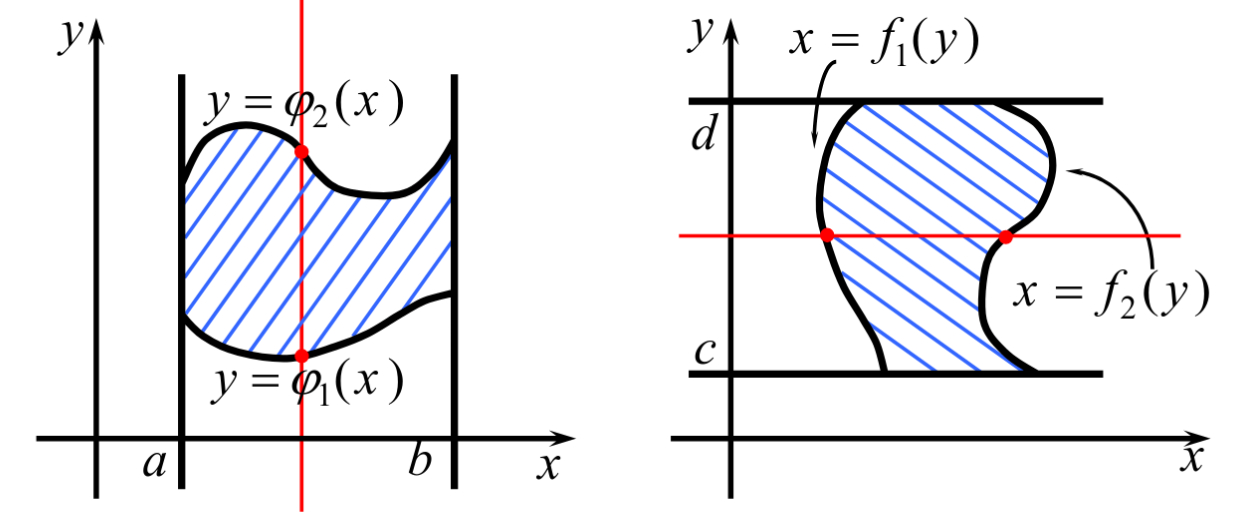
\includegraphics[width=\textwidth]{includes/right}
\end{figure}

Двойной интеграл вычисляется сведением к повторному интегралу.

Сведение двойного интеграла к повторному рассмотрим на примере геометрической интерпретации двойного интеграла как объема цилиндрического бруса.

Предположим, что область интегрирования $(S)$ --- правильная в направлении оси $Oy$ и ограничена линиями $y = y_1(x)$, $y = y_2(x)$, $x = a$ и $x = b$.

Пусть площадь сечения тела плоскостью, отвечающей абсциссе $x$ и перпендикулярной оси $Ox$, равна $\sigma(x)$.

Тогда объем тела, если он существует, равен
\[
  V = \int_a^b \sigma(x) dx, \quad \text{где} \quad \sigma(x) = \int_{y_1(x)}^{y_2(x)} f(x, y) dy.
\]

С другой стороны, объем тела равен
\[
  V = \iint_S f(x, y) dxdy.
\]

Следовательно, вычисление двойного интеграла сводится к последовательному вычислению двух определенных интегралов:
\[
  \iint\limits_{(S)} f(x,y) dxdy = \int\limits_{a}^{b} dx \int\limits_{y_1(x)}^{y_2(x)} f(x,y) dy.
\]

Указанная формула справедлива, если $f(x, y)$ интегрируема на области $(S)$, ограниченной линиями $y = y_1(x)$, $y = y_2(x)$, $x = a$, $x = b$, и $\forall x \in [a, b]$ существует внутренний интеграл
\[
  \int\limits_{y_1(x)}^{y_2(x)} f(x,y) dy.
\]

Аналогично, если $f(x, y)$ интегрируема на области $(S)$, правильной в направлении оси $Ox$ и ограниченной линиями $x = x_1(y)$, $x = x_2(y)$, $y = \alpha$, $y = \beta$, и $\forall y \in [\alpha, \beta]$ существует внутренний интеграл
\[
  \int\limits_{x_1(y)}^{x_2(y)} f(x,y) dx,
\]
то
\[
  \iint\limits_{(S)} f(x,y) dxdy = \int\limits_{\alpha}^{\beta} dy \int\limits_{x_1(y)}^{x_2(y)} f(x,y) dx.
\]

Если область $(S)$ правильная, то справедливы обе формулы и
\[
  \int\limits_{a}^{b} dx \int\limits_{y_1(x)}^{y_2(x)} f(x,y) dy = \int\limits_{\alpha}^{\beta} dy \int\limits_{x_1(y)}^{x_2(y)} f(x,y) dx.
\]

\section{Замена переменных в двойном интеграле.}
Пусть в двойном интеграле \(\iint\limits_D f(x,y)ds\) требуется перейти к новым переменным \(u,v\),
по формулам \(x=x(u,v)\), \(y=y(u,v)\), \((u,v)\in D^*\). Функции \(x=x(u,v)\), \(y=y(u,v)\) непрерывны в \(D^*\)
вместе со своими частными производными и осуществляют взаимно-однозначное
отображение \(D^*\) на \(D\), т.~е. существуют обратные функции \(u=u(x,y)\), \(v=v(x,y)\), \((x,y)\in D\).

Формула замены переменной в двойном интеграле имеет вид:
\[
  \iint\limits_D f(x,y)ds = \iint\limits_{D^*} f(x(u,v),y(u,v))|J|ds^*, \quad \text{где } D^* -
\]
образ \(D\) в системе \(Ouv\). Определитель \(J\) называют якобианом преобразования
координат. Если якобиан не равен нулю, то преобразование \(D \leftrightarrow D^*\) имеет смысл (в таком
случае говорят, что оно невырожденное).
\section{Полярные координаты. Вычисление двойных интегралов в полярной системе координат.}
Рассмотрим частный случай. Пусть нужно записать двойной интеграл

\[
  \iint_D f(x, y) dxdy
\]

в полярной системе координат, если полярная ось \( l \) совмещена с осью \( OX \), а полюс --- с началом координат, т.~е.

\[
  \begin{cases}
    x = r\cos\varphi, \\
    y = r\sin\varphi.
  \end{cases}
\]

В этом случае \( u=r, v=\varphi \),

\[
  J =
  \begin{vmatrix}
    \frac{\partial x}{\partial r} & \frac{\partial x}{\partial \varphi} \\
    \frac{\partial y}{\partial r} & \frac{\partial y}{\partial \varphi}
  \end{vmatrix}
  =
  \begin{vmatrix}
    \cos\varphi & -r\sin\varphi \\
    \sin\varphi & r\cos\varphi
  \end{vmatrix}
  = r\cos^2\varphi + r\sin^2\varphi = r > 0
\]

и \( ds = drd\varphi \) --- элемент площади в полярных координатах.

Тогда имеет место формула перехода к полярным координатам в двойном интеграле

\[
  \iint_D f(x, y) dxdy = \iint_{D'} f(r\cos\varphi, r\sin\varphi) r dr d\varphi.
\]
\section{Сформулируйте определение тройного интеграла и его основные свойства.}
Пусть в ограниченной замкнутой пространственной области $T$ задана непрерывная функция $f(x, y, z)$.
Разобьём эту область произвольным образом на $n$ частичных пространственных ячеек с объёмами $\Delta V_k$.
В каждой ячейке выберем по одной произвольной точке $P_k(x_k, y_k, z_k)$ и вычислим значение функции
во взятых точках. Составим интегральную сумму вида:

\begin{equation}
  \delta = \sum_{k=1}^{n} f(P_n) \Delta{V_n}
\end{equation}

Тройным интегралом от функции по области называется предел интегральных сумм при стремлении к нулю наибольшего из диаметров всех ячеек данного разбиения

\begin{equation}
\iiint\limits_T f(P) dV =  \max\limits_\text{$1 \leq k \leq n$} \lim_{\Delta V_k \to o} \sum_{k=1}^{n} f(P)) \Delta{V}
\end{equation}

Свойства тройного интеграла:
\begin{enumerate}
\item Линейность
  Если f(P) и g(P) интегрируемы в T, то их линейная комбинация также интегрируема
  \begin{equation}
    \alpha \iiint\limits_T f(P) dV + \beta \iiint\limits_T g(P) dV = \iiint\limits_T \alpha f(P) + \beta g(P) dV
  \end{equation}
\item Аддитивность
  Если область $T$ разбита на две подобласти $T_1$ и $T_2$ без общих внутренних точек
  ($T = T_1 \cup T_2$, $T_1 \cap T_2 = \emptyset$), то:
  \begin{equation}
    \iiint\limits_T f(P) \, dV =
    \iiint\limits_{T_1} f(P) \, dV +
    \iiint\limits_{T_2} f(P) \, dV
  \end{equation}
\item Неотрицательность
  Если f(x, y) интегрируема в T и $f(P) \geq 0$ в T, то
  \begin{equation}
    \iiint\limits_T f(P) dV \geq 0
  \end{equation}
\item Монотонность
  Если $f(P) \leq g(P)$ для всех $(P) \in T$, то:
  \begin{equation}
    \iiint\limits_T f(P) dV \leq \iiint\limits_T g(P) dV
  \end{equation}
  В частности, если $f(P) \geq 0$ на $T$, то:
  \begin{equation}
    \iiint\limits_T f(P) \, dV \geq 0
  \end{equation}
\item Оценка интеграла по модулю
  Если f(x, y) интегрируема в T, то |f(P)| интегрируема в T
  \begin{equation}
    |\iiint\limits_T f(P)dV|  = \iiint\limits_T |f(P)| dV
  \end{equation}
\end{enumerate}
\section{Вычисление тройного интеграла в прямоугольной декартовой системе координат.}
Вычисление тройного интеграла сводится к вычислению определенного и двойного интегралов.
Будем рассматривать область $(V)$, правильную в направлении оси $O_z$, т.~е. такую, что любая прямая, проходящая через внутреннюю точку области параллельно оси $O_z$, пересекает границу области в двух точках. Пусть область $(V)$ ограничена сверху и снизу поверхностями $z = z_1(x, y)$ и $z = z_2(x, y)$ соответственно, а также цилиндрической поверхностью $F(x, y) = 0$ с образующими, параллельными оси $O_z$.

$(D_{xy})$ --- проекция $(V)$ на плоскость $Oxy$. Функция $f(x, y, z)$ непрерывна в области $(V)$. Тогда справедлива формула

\[
\iiint\limits_{(V)} f(x, y, z) dxdydz = \iint\limits_{(D_{xy})} dxdy \int\limits_{z_1(x, y)}^{z_2(x, y)} f(x, y, z) dz.
\]

Если при этом область $(D_{xy})$ --- правильная в направлении оси $Oy$ и определяется следующими неравенствами: $a \leq x \leq b$, $y_1(x) \leq y \leq y_2(x)$, то тройной интеграл может быть вычислен по формуле

\[
\iiint\limits_{(V)} f(x, y, z) dxdydz = \int\limits_{a}^{b} dx \int\limits_{y_1(x)}^{y_2(x)} dy \int\limits_{z_1(x, y)}^{z_2(x, y)} f(x, y, z) dz.
\]
\section{Цилиндрические координаты. Вычисление тройных интегралов в цилиндрической системе координат.}
Gереход к цилиндрическим координатам $\varphi$, $\rho$ и $z$ по формулам $x = \rho \cdot \cos\varphi$, $y = \rho \cdot \sin\varphi$, $z = z$, где $\rho \geq 0$, $0 \leq \varphi < 2\pi$, $-\infty<z<\infty$.

Якобиан замены

\[
J(\rho, \varphi, z) =
\begin{vmatrix}
  \frac{\partial x}{\partial \rho} & \frac{\partial x}{\partial \varphi} & \frac{\partial x}{\partial z} \\
  \frac{\partial y}{\partial \rho} & \frac{\partial y}{\partial \varphi} & \frac{\partial y}{\partial z} \\
  \frac{\partial z}{\partial \rho} & \frac{\partial z}{\partial \varphi} & \frac{\partial z}{\partial z}
\end{vmatrix}
=
\begin{vmatrix}
  \cos \varphi & -\rho \sin \varphi & 0 \\
  \sin \varphi & \rho \cos \varphi & 0 \\
  0 & 0 & 1
\end{vmatrix}
= \rho.
\]

Таким образом, при переходе к цилиндрическим координатам получаем

\[
\iiint\limits_{(V)} f(x, y, z) dxdydz = \iiint\limits_{(V')} f(\rho \cos \varphi, \rho \sin \varphi, z) \rho d\rho d\varphi dz.
\]
\section{Сформулировать необходимый признак сходимости числового ряда.}
Елси числовой ряд $\sum_{k=1}^{n}a_k$ сходится, то $\lim_{k \to \infty} a_k = 0$
\section{Достаточные признаки сходимости знакоположительных числовых рядов: сформулировать признак сравнения.}
Числовой ряд с положительными членами сходится, если его члены заведомо не превосходят членов другого зоведомо сходящегося ряда. Ряд расходится если его члены превосходят члены другого заведомо сходящегося ряда.
\begin{equation}
\begin{aligned}
  &\sum_{k=1}^{\infty} a_k \quad a_k = 0 \quad \sum_{k=1}^{\infty} b_k \quad b_k = 0 \\
  &\exists n \in \mathbb{N} : \forall k \geq n \quad a_k \leq b_k \quad \\
  &\text{Тогда: } \\
  &\sum_{k=1}^{\infty} b_k \text{сходится} \implies \sum_{k=1}^{\infty} a_k \text{сходится} \\
  &\sum_{k=1}^{\infty} a_k \text{расходится} \implies \sum_{k=1}^{\infty} b_k \text{расходится} \\
\end{aligned}
\end{equation}
\section{Достаточные признаки сходимости знакоположительных числовых рядов:сформулировать предельный признак сравнения и следствие из него.}
Если два числовых ряда с положительными членами $\sum_{k=1}^{\infty} a_k \quad a_k  \geq 0 \quad \forall k \in N$ и $\sum_{k=1}^{\infty} b_k \quad b_k > 0$ справедливо соотношение $\lim_{k \to \infty} \frac{a_k}{b_k} = c \quad 0 < c < \infty $, то эти ряды сходятся и расходятся одновременно.
\section{Достаточные признаки сходимости знакоположительных числовых рядов:сформулировать предельный признак Даламбера.}
Пусть для ряда с положительным членами  $\sum_{k=1}^{\infty} a_k \quad a_k > 0 \quad \forall k \in N \quad \exists \lim_{k \to \infty} \frac{a_{k+1}}{a_k}  = q \quad q \geq 0 $, тогда:
\begin{enumerate}
\item Если q < 1, то ряд сходится;
\item Если q > 1, то ряд расходится;
\item Если q = 1, поведение ряда нельзя определить этим признаком
\end{enumerate}
\section{Достаточные признаки сходимости знакоположительных числовых рядов:сформулировать предельный радикальный признак Коши.}
Пусть для ряда с положительным членами  $\sum_{k=1}^{\infty} a_k \quad a_k  \geq 0 \quad \forall k \in N \quad \exists \lim_{k \to \infty} \sqrt[k]{a_k}  = q $, тогда:
\begin{enumerate}
\item Если q < 1, то ряд сходится;
\item Если q > 1, то ряд расходится;
\item Если q = 1, оведение ряда нельзя определить этим признаком
\end{enumerate}
\section{Достаточные признаки сходимости знакоположительных числовых рядов:сформулировать интегральный признак Коши.}
Пусть функция f(x) действительна, неотрицательна и непрерывна в некотором промежутке $[m; +\infty )$ не возрастает в этом промежутке. Тогда для сходимости ряда $\sum_{k=1}^{\infty} f(k)$ необходимо и достаточно, чтобы сходился несобственный интеграл $\int_{m}^{\infty}f(x)dx$.
\section{Дать определение условно сходящегося числового ряда. Сформулировать признак Лейбница.}
Знакочередующийся ряд  - действительный ряд у которого соседние члены имеют разные знаки
\begin{equation}
\sum_{k=1}^{\infty}(-1)^{k+1} a_k \quad a_k > 0
\end{equation}
Пусть Знакочередующийся ряд
\begin{equation}
\sum_{k=1}^{\infty}(-1)^{k+1} a_k \quad a_k > 0  \quad \forall k \in N
\end{equation}
удовлетворяет условиям
\begin{enumerate}
\item $a_1 \geq a_2 \geq a_3 \geq a_4 \geq \text{...} \geq a_k \geq \text{...}$
\item  $\lim_{k \to \infty} a_k = 0$
\end{enumerate}
Тогда ряд сходится.

Если ряд удовлетворяет условия признака Лейбница
\begin{enumerate}
\item $0 < S < a_1$
\item модуль суммы всякого его остатка останется $R_n$ оценивается сверху числом $a_{n+1}$
  \begin{equation}
    |R_n| = | \sum_{k=n+1}^{\infty} (-1)^{k+1} a_k | < |a_{n+1}| \quad \forall n \in N
  \end{equation}
\end{enumerate}
\end{document}